\chapter{Background}\label{ch:Background}

\begin{mynote}
%\vspace{0.5cm}
\subsubsection{Chapter outline}
In this chapter, I first review previous literature on interruptions, and discuss existing interventions to manage interruptions. The second section discusses research related to seeking information as part of work. The last section focuses on prior data entry research. 
%\vspace{0.2cm}
\end{mynote}

%The aim of this thesis is to understand how the disruptiveness of inquiries, with different time costs, for a data entry task can be reduced. 
This chapter provides an overview of previous literature to situate my research on self-interruptions to look up information for data entry. The chapter consists of three sections: I first consider prior research on interruptions, and discuss existing interventions to manage interruptions. This section provides context to the problem of interruptions in the workplace and its effect on task performance, and what factors influence the disruptiveness of interruptions. The section also shows the advantage of using a combination of qualitative and quantitative research methods to study interruptions: while qualitative methods are needed to get an understanding of the type of interruptions that occur and in which context, experiments have been a suitable method to then understand how certain factors influence the disruptiveness of interruptions on task performance. The review of existing interruption management tools gives insight into how other types of interruptions have been managed, and I draw on similarities and differences between inquiries in particular and interruptions in general to argue why current tools are insufficient to support inquiries. The second section discusses research related to managing information as part of work, which demonstrates that the way in which people interrupt to look up information depends on the nature of the task and work. Existing tools to support information management have mostly focused on tasks where information has already been collected and needs to be organised, but does not consider how best to interrupt a task when additional information is needed. The last section focuses on prior data entry research, which highlights that design interventions can reduce data entry errors, but need to be adapted to be suitable for disruptive work environments. 

\section{Terminology}
Throughout the thesis, I use the key terms inquiries, interruptions, time cost and information access cost. To avoid confusion, I clarify the definitions of these terms here.

\textit{Inquiries} are a type of self-interruption, and happen when a person goes away from a task, to look up information that aids the completion of that primary task \citep{Jin2009}. This type of interruption is the main focus of the thesis. In sections where the terms \textit{interruptions} or \textit{self-interruptions} are used, rather than inquiries, it can be assumed this section refers to all types of interruptions. 

\textit{Time costs} refer to the time involved to complete an action. Prior studies in cognitive psychology have used the term \textit{information access cost}, which  is a particular type of time cost, and refers to the time, physical and/or mental effort required to access information \citep{Gray2006}. Because this thesis looks at a broader definition of time costs to look up information, which can be caused by accessing information, but also searching for information and getting distracted by other information, the term time costs is used for the majority of the thesis. When the term information access cost is used, usually when discussing prior work, it refers to the specific time cost of accessing information. 

\section{Interruptions and fragmentation of work}
%Occurrence of interruptions
Computer work frequently gets interrupted: on average, office workers switch between activities every three minutes \citep{Gonzalez2004}. Furthermore, tasks themselves are also often fragmented: people have to switch between documents and applications to look up information for their task. These interruptions can be disruptive: it can slow people down, increase errors and cause stress. However, some interruptions can also be beneficial: short breaks can improve mood and restore energy \citep{Mark2014a}, and quickly retrieving relevant information can aid completion of a task \citep{Jin2009}. A range of both field studies and controlled experiments have tried to understand what factors influence disruptiveness of interruptions.

\subsection{Interruptions during computer work}
%To understand some of the reasons and underlying mechanisms of interruption behaviour, interruptions have both been studied through field studies and controlled experiments.

%Self-interruptions are harder to manage
Field studies have been done to understand interruptions in situated settings such as healthcare \citep[e.g.][]{Grundgeiger2010, Westbrook2010} and office environments \citep[e.g.][]{Czerwinski2004, Gonzalez2004}. For the scope of this thesis, I mainly discuss work on interruptions during computer-based work. \citet{Mark2005} observed office workers, and found half of all interruptions are self-interruptions, and that self-interrupted tasks were less likely to be resumed later than tasks that were stopped by an external interruption. An interview study on interruption management strategies found major differences in the level of difficulty for users to manage external versus self-interruptions \citep{Kim2017}. Whereas external interruptions may be ignored or deferred, self-interruptions require more self-control, and are experienced as harder to resist and as more distracting. Furthermore, self-interruptions take more time to recover from than external interruptions as they can end up taking much longer than planned. When switching between computer windows, there are numerous opportunities to get distracted and get diverted from the main task. For example when switching to communication tools, users can get tempted to answer unrelated messages instead \citep{Mark2012}. 

%Individual differences
There are also individual differences in people's tendency to attend to distractions and resist interruptions \citep{Lyngs2018, Mark2016a}. \citet{Mark2016a} conducted a field study with office workers, in which window switching behaviour was measured, and participants were asked to fill in a personality survey at the end of each day. They found a positive relationship between how people scored on a Neuroticism and Impulsivity scale, their switching behaviour, and how productive they felt at the end of the day. This suggests that distractibility could be a personal trait.

 %Types of self-interruptions
\citet{Jin2009} conducted a observational study of self-interruptions during computer tasks. They identified seven categories of self-interruptions: adjustments, breaks, recollections, routines, triggers, waits, and inquiries. Adjustments happen when people try to adjust and improve their work environment, for example by closing irrelevant documents. Breaks are moments when people switch to something else because they want to take a rest from the main task. Recollections occur if people remember they need to perform another task. Routines are self-interruptions that happen out of habit, such as checking social media regularly. A trigger is an external stimulus that triggers the user to switch to another task. Waits are when people switch to something else during a delay in the primary task. Lastly, an inquiry, which is the type of interruption I focus on in this thesis, happens when a person goes to look up information to aid the completion of a primary task. Some of these interruptions may have a positive effect. For example, breaks can be positive: ICT is increasingly used in work breaks, and these self-interruptions may restore energy \citep{Skatova2016}. Furthermore, in Jin and Dabbish's study inquiries positively impacted people's work, as they quickly found what they were looking for. However, Jin and Dabbish speculate that these interruptions may be disruptive if information cannot be found straight away. Overall, all types of interruptions may become disruptive if they happen too often or for too long.

%Effect on task performance
Given the occurrence of interruptions, studies have tried to understand the consequences of interruptions on work productivity. Studies focusing on university students found that students who made fewer interruptions to social media during class and study sessions had higher grades \citep{Carrier2015}. While grades can be used to measures students' performance, it is more difficult to objectively measure productivity in the workplace, and most workplace studies have relied on participants' self-assessment of productivity. For example, \citet{Mark2015} instructed participants to assess how productive they felt on a 7-point Likert scale. %\citet{Mark2016} constructed a more expanded index of productivity that consists of six dimensions: accomplishment, efficiency, satisfaction, effectiveness, quality and overall assessment of work. Participants in their study were asked to respond to a number of statements such as "How much did you accomplish today based on what you had planned to accomplish?" Responses were measured on a 7-point Likert scale. These responses were combined to construct an index of productivity. 
Self-assessments of productivity were then compared with objective measures of people's screen switches, which were obtained using logging techniques. It was found that the more screen switches people made, the less productive they felt at the end of the day \citep{Mark2015}, and . 
These studies suggest that fragmented attention has a negative effect on work productivity, though to study a direct relationship between interruptions and work performance, experiments have been used, which will be discussed next. 

\subsection{Experimental investigations of interruptions}
%Controlled experiments
Field studies have given insight in the prevalence of interruptions, the context that leads up to an interruption, and the different type of interruptions that happen. A limitation of the method is that it is difficult to establish a direct link between various factors influencing the disruptiveness of interruptions. Controlled experiments on the other hand are a useful method to measure the effect of interruptions on task performance.

%Length and timing of interruption
Two factors that contribute to the disruptiveness of an interruption are its length and timing. This can be explained by the Memory for Goals theory \citep{Altmann2002}: this theory holds that when people are interrupted from a task, the representation of the task in working memory enables them to keep track of where they were in the task, making it easier to resume. The longer people are interrupted and away from a task, the more likely that this representation weakens and fades from memory \citep{Altmann2017, Monk2008}. Furthermore, it is more disruptive if people are interrupted at high than low workload moments, because people have to hold more information in memory while being interrupted. For instance, interruptions have been shown to be more disruptive if they happen in the middle of a subtask compared to when they happen between subtasks, because people have a higher workload of remembering where they are in the middle of the subtask \citep{Gould2013a, Iqbal2005}. \citet{Salvucci2010} conducted an experiment investigating how people manage interruptions that are deferrable, and found people deferred interruptions until moments of low workload. This suggests that people may be fairly good at focusing on a task and postponing interruptions, though the study only looked at external interruptions, which were triggered by notifications. As discussed above, self-interruptions are perceived to be harder to ignore than external interruptions. Furthermore, in Salvucci and Bogunovich's study people did not have to remember to attend to a task later, and had their working memory free to continue to focus on the main task. Self-interruptions, on the other hand, are often triggered by the users' internal thought \citep{Jin2009}: holding the intention to interrupt in working memory may be just as cognitively effortful as interrupting a task at a high-workload moment.

%Relevance of an interruption
Interruptions can be useful if they benefit the task \citep{Jin2009}, and a range of studies have shown that irrelevant interruptions are more disruptive than relevant ones \citep{Adamczyk2004, Gould2013a}. Based on this finding, it may seem more important to focus on avoiding irrelevant interruptions. However, task-relevant interruptions can be just as distracting and disruptive if not managed well. \citet{Iqbal2008} conducted a study, in which participants were interrupted by relevant or irrelevant notifications during work. Even though participants wanted relevant interruptions to happen more often than irrelevant interruptions, for both types of interruptions participants were observed entering chains of diversions. This refers to moments where the participant does not return to the main task after an interruption, but instead attends to other activities. This means that both relevant and irrelevant interruptions may trigger people to spend longer on interruptions than necessary.

\subsection{The effect of information access costs on interruptions}
%IAC
People’s interruption behaviour is further influenced by time costs associated with making an interruption. Several studies have looked at how information access costs (IAC), that is the physical, mental and cognitive effort to access task information, influence how people switch away from a task to look up task information. Even though most of these studies do not explicitly label these switches as 'interruptions', window switches can still be disruptive \citep{Rule2013}. In a typical IAC study, participants are asked to complete an experimental task, such as solving the Tower of Hanoi puzzle \citep{Waldron2007}, programming a VCR \citep{Gray2004} or copying a pattern of coloured blocks \citep{Gray2006}. To complete the task, the participant needs to access task information. In the control condition, this information is easily accessible. In experimental conditions, there is a cost to access the information, for example the information is covered by a grey mask, and participants have to hover over the mask with their cursor to reveal the information. A consistent finding across IAC research is that if the cost to access task information increases, people try to minimise time costs by making fewer switches to the information source, and instead rely on information in memory. This adaptive use of memory is explained by the soft constraints hypothesis \citep{Gray2006}, a cognitive theory which holds that people adapt their cognitive strategies to the constraints of a task environment with the aim to optimise task completion time: rather than preserving cognitive resources, people try to minimise time.

Though a memory-based strategy carries the risk that the memorised information is incorrect, several studies have shown that an increased IAC can also have a positive effect on task performance. In a problem-solving task, an increased IAC resulted in people taking the time to carefully memorise task information and plan actions before making any moves, which made them more efficient in completing the task \citep[e.g.][]{Morgan2007, Morgan2012}. A memory-intensive strategy can also be useful for resuming a task after an interruption. \citet{Morgan2009} conducted a study looking at the effect of IAC on a copying task. People had to perform the Blocks World Task (BWT), which involves copying a pattern of coloured blocks, by dragging blocks from a resource window to a target window. They manipulated the cost to access the original source which showed the pattern they had to copy. In the Low IAC condition, the pattern was permanently visible on the screen. In the Medium IAC condition, the pattern was covered by a grey mask and participants had to hover over the mask with their mouse to reveal the pattern. In the High IAC condition, there was an additional time delay before the pattern was revealed. At certain intervals, they would get interrupted and asked to do a secondary task, irrelevant to the primary task. As IAC increased, people made fewer but longer visits to the target pattern and memorised more of the pattern. As a result, following the irrelevant interruption they were faster to resume the primary task, and could copy more blocks before having to revisit the target pattern. This again shows how a strong representation of the task in working memory aids resumption after an interruption.

%Limitation IAC studies
The soft constraints hypothesis assumes a situation where the user only makes switches between task information and the main task. In this context, a longer interruption time may be used to encode task information in memory, with the effect that people are quicker to resume a task and more efficient to complete it \citep{Morgan2007, Morgan2012}. In reality, people may need to make several window switches before they retrieve the right information, and people may further switch to other unrelated tasks. In this context, a long interruption time may be caused because people are diverted by other tasks and not attending to the task at all \citep{Iqbal2008}, which can increase errors. As such, while the theory is useful in explaining how people adapt their use of memory to information access costs, it is difficult to map the theory to a broader range of time costs of interruptions in the workplace. 

\subsection{Interruption management tools}
Given the occurrence of interruptions and its potential negative effect on work performance, there have been different approaches to support self-interruption management and improve people's focus. 

%Giving reflective information
Commercial applications, such as RescueTime and ManicTime, provide users with an overview of all their computer activities, to increase awareness of their use of time. Users can view how much time they spent in particular documents, websites and applications, and during which hours of the day. Little work has evaluated how effective these applications are in improving focus, and interview studies have reported a lack of engagement among users \citep{Collins2014, Whittaker2016}. An interview study by \citet{Collins2014} on understanding people’s use of RescueTime found four barriers to explain people’s lack of engagement with the data: the data lacks salience, a lack of context made it difficult to extract work patterns from the data, participants felt it was not a true representation of their actual activities, and they were not sure what actions to take based on the data. 

\citet{Whittaker2016} interviewed office workers and students to establish user requirements for a time awareness application, and found users were primarily interested in their current activities rather than long-term behaviour. Therefore, they developed and evaluated an application which presented users with a visualisation of the last 30 minutes of computer activity. The application reduced the time spent in email, browsing and social media, but it did not increase time spent on work and it was unclear whether it improved people’s productivity. Whittaker et al. speculated that participants may already have time limits to spend on work, but are more flexible with the amount of time they spend on other online activities.

%Blocking distractions
Other commercial tools such as StayFocusd, Freedom and FocusMe limit access to specific sources. \citet{Kim2017} developed an intervention that allowed people to block applications and websites across devices for a fixed period that they considered distracting. The blocking feature was viewed positively by participants who found it difficult to mitigate self-interruptions themselves. However, many distracting sources, such as web browsers and instant messaging applications, can not be blocked during work because these need to be accessed for the current work task. To investigate how appropriate a blocking approach would be in the workplace, \citet{Mark2018} conducted a field study with office workers using blocking software for one week. Participants installed software that allowed them to disable websites, and were asked to block any websites they considered distracting and nonessential to work. Several participants disliked the feeling that the software was controlling them, and rather wanted to learn how to gain control themselves over their work and interruptions.

Other interventions suggest giving participants information during a specific task may help focus. \citet{Gould2016a} looked at people’s switches to unrelated activities during an online data entry task. They found that an intervention that encouraged people to stay focused after they had self-interrupted reduced the number of switches to unrelated tasks. 

\subsection{Summary}
Interruptions in the workplace are common, and both controlled and field studies have found a link between fragmented attention and a decrease in work performance \citep{Bailey2001, Carrier2015}. Various tools have been developed aiming to reduce interruptions and digital distractions, but do not consider interruptions which are required for work, such as looking up task-related information. 

\section{Managing information needs}
%\subsection{Occurrence of looking for information}
Though applications are usually designed assuming users stay within a single application for a task, task information is often spread across sources, which requires users to interrupt their work and switch between multiple applications and documents to retrieve information \citep{Cangiano2009, Czerwinski2004, Mark2005, Sellberg2014}. To get a better understanding of how users can be supported in this fragmentation of work, a line of studies have studied how people find and re-find information as part of work in healthcare \citep{Reddy2002} and law offices \citep{Cangiano2009, Makri2008}, on a mobile device \citep{Sohn2008}, and how information behaviour differs for different types of tasks \citep{Bondarenko2005}. For the purpose of this thesis, I limit my discussion to how information needs are addressed in practice to aid completion of a particular task or work, rather than theoretical models of information seeking as a task in itself.

\subsection{Managing inquiries for work}
Several studies have used interviews and observations to get a detailed understanding of people's information behaviour at work. For instance, \citet{Reddy2002} conducted an ethnographic study in an intensive care unit of a hospital. The focus of this study was on how health-care workers managed and retrieved the information sources needed to support their work throughout the day. Health-care workers used their own and their colleagues' working patterns to plan for future information needs. This planning was necessary because of the nature of work: workers were on the move for most of their working day, they had to get information sources from different locations within the unit, and were reliant on other people to get access to information. These physical constraints and dependencies encouraged workers to think about whether to collect information right away, postpone it until later, or strategically request it for later access. In contrast, office workers are often situated behind a desk, and information may be only a few clicks away. It is unclear whether office workers also engage in this kind of planning behaviour. \citet{Cangiano2009} interviewed and observed people in law offices searching for information. They found that lawyers do not plan for future information needs, but instead have to spend time retracing the steps of a legal case, and that they need to access different sources to find all the relevant information for the case, such as emails, instant messages with colleagues, legal documents, and written reports. They argue that, even though work may appear fragmented, these participants still perceived they were working on the same activity when switching between all these different sources.

\subsection{Factors influencing inquiries}
 %People do not always realise they need certain information until they have started a task. Leaving the primary task interface to look up this information does not have to be bad if it is useful for the current activity, but resuming the primary task after this interruption still takes time \citep{Rule2013}. 
While some studies have observed people planned inquiries carefully around their work \citep{Reddy2002}, other studies have shown that people interrupt their task immediately as soon as they think of information they need \citep{Jin2009}.
To get insight into what factors may influence information behaviour, \citet{Sohn2008} conducted a diary study investigating how people address inquiries on a mobile phone. They did not focus on a particular task, but asked participants to keep a record of all instances where they needed information for an activity they were doing.  Four main factors determined whether participants looked up the information immediately or whether they postponed to address it later: urgency, importance, situational factors, and costs. The more urgent and important it was to have the information for the activity they were doing, the more likely it was they looked up the information at the moment they realised they needed it. If they were currently involved in an activity that made it difficult to address the information need at that moment, or they did not know where to get the information from, they were more likely to postpone the inquiry. Lastly, the more time or monetary cost was associated with getting the information, the more likely they were to not address it or leave it until later. This suggests that time costs may make people less likely to interrupt a task, although Sohn et al.’s study exclusively looked at information needs on a mobile device, which differs from desktop search: the affordance of easy switching between windows on conventional desktop computers may give the false impression that information is easier to access \citep{Sellen2003}. Furthermore, participants mostly reported non-work situations in which information was not essential: the majority of information needs were categorised as 'trivia'. As such, participants may have been more likely to give up an information search if it required effort, compared to if this search was required for work: for 30\% of the diary entries information was not accessed later at all, with the main reason being that it was unimportant. 

\subsection{Types of tasks}
The way in which people address inquiries is further influenced by the type of task. \citet{Bondarenko2005} distinguish between two different types of tasks that information workers engage in: administrative and research tasks. Administrative tasks are routine tasks, of which the steps are usually the same, and are characterised by short and frequent switches between documents. For these tasks, documents often switch between what Bondarenko \& Janssen refer to as 'hot', when a document is needed, and 'cold', when a document is not needed and archived. For administrative tasks, documents are only needed for a short period of time, but need to be accessed repeatedly. Examples are filling in a personal information form for a new member of staff. Research tasks, on the other hand, only require a small number of documents, but these need to be accessed for a longer period of time. An example is writing a research paper: the writer may need to consult another paper, and need to read this or keep it close by for a long period of time.

Because of the different nature of these tasks, they need different support. \citet{Bondarenko2005} conclude that most information management tools support 'pure' administrative tasks, which are repetitive, structured and predictable, but provide inadequate support for research tasks. However, these two task types should be seen as two extremes rather than a distinct classification, and many tasks may fall somewhere on the spectrum between these two extremes. For example, though data entry shares some of the characteristics of an administrative task and usually follows the same sequence of steps, it does not always follow the same linear path, and as will be demonstrated in the next chapter of this thesis, it does not always require the same information. 


\subsection{Information management tools}
Given the fragmented nature of many tasks, several tools have looked at how to make information easier to access and reduce interruptions, so people can focus on their work. For example, GroupBar \citep{Smith2003} makes it possible to group windows needed for a task in the task bar. \citet{Cangiano2009} developed ActivityTrails, a tool which allows people to play back a visual summary of sources which were accessed the last time they were working on an activity.  These tools can be useful for work which has to be resumed later on, in which the same sources need to be accessed again, but may be less useful when starting a new activity, in which new sources are needed.

Increased screen space has also been explored as a way to support people in fragmented work, as people will not need to flick back and forth between windows as often, but can have these open and on the screen simultaneously \citep{Czerwinski2003}.  \citet{Bi2009} conducted a week-long diary study looking at how office workers utilise a large screen and a second screen to access information. People arranged information on their available screen space differently in each condition. For two screens, people dedicated one screen for their primary task which filled up the entire screen. They moved all information they did not need at the moment to the second screen and did not bother re-arranging the windows: they would only attend to the second screen when they needed information, and deliberately allocated the second screen for a different purpose than the first screen. For one large screen, participants first spent a certain amount of time optimising the layout of the windows by resizing and re-arranging them. They put all windows needed for the primary task in the center of the screen and placed other windows in the periphery.  As participants needed information from this periphery, they dragged the window to the center of the screen rather than interacting with that particular part of the screen. On the other hand, if participants needed information from the second screen, they physically turned to the second screen and interacted with it but did not drag the information to the primary screen, unless they had to interact with it for a longer time.

Though people had to spend some initial time organising information, office workers felt more focused on the task and immersed in their work when surrounded by task-relevant documents. In this study, participants were given large screens for the purpose of the study, so there may have been a novelty effect. In practice, dual screens have been shown to also increase multitasking and fragmented attention \citep{Robertson2005}. In addition, a large screen may reduce the disruption of switching between windows but it can introduce another type of access cost, which \citet{Robertson2005} refer to as the \textit{'distal information access cost problem'}: as screen size increases, it becomes harder and more time-consuming to target and select certain buttons and windows. 

Despite the popularity of one large screen, \citet{Grudin2001} states dividing screen space up in multiple monitors can sometimes be better. He argued that the main benefit of having a second screen is not so much the increase in screen space, but the partitioning of information into dedicated areas: having multiple screens prompts people to think more about where to put which information. To support his argument, he conducted a field study looking at how office workers use multiple screens to arrange information. Participants positioned information they did not need at the moment on a second screen where they were not distracted by it, but could easily access it when needed. People preferred that information was always in the same known location and referred to the second screen whenever they needed to look information up, even when they were aware they could also access it using their primary screen as well, where the information was sometimes less time-consuming to access \citep{Grudin2001}. 

\subsection{Summary}
Many computer tasks require switching between different documents, applications and windows. How people switch depends on the type of task, the cost to access information, the urgency and importance of an information need, and the current situation people are in. Several tools have tried to make it easier to group information and search, so people can focus on the main task. However, these solutions are best suited for situations where information is known beforehand and needs to be re-used, and does not consider how best to interrupt a task when additional information is needed. An increased screen size can reduce certain access costs, such as mouse clicks to flick back and forth between windows, but may introduce other access costs, such as time to select the right window, and increase multitasking to unrelated tasks.

\section{Data entry}
%Occurrence of data entry
The way in which people interrupt to look up information can depend on the type of task \citep{Bondarenko2005}, so in order to get a detailed understanding of interruption behaviour, it is not only important to consider the task environment but also the scope of the task studied. This thesis focuses specifically on data entry, a core computing task in office scenarios. An example of a data entry task is completing a payment request form, in which information has to be entered into specific fields of the form, such as the person's name, address, and bank account details. Interruptions during this type of task can be particularly disruptive as it not only takes time to resume the task, but it can also increase data entry errors. The consequences of data entry errors can range from an inconvenience to having a more serious outcome: in 2018, up to 1,500 junior doctors' job offers in the UK were withdrawn after a data entry error in a spreadsheet caused the candidates to incorrectly receive a job offer \citep{BBC2018}. It is therefore important to study how errors can be reduced, and a line of experiments have looked at understanding the different steps of a data entry task, and have demonstrated how making design changes to a data entry interface can reduce errors. 
 
%While prior work has studied the phenomenon of fragmented office work and self-interruptions during computer activities, it has generally not focused on a specific task. 

A data entry task can be broken down in four stages, as is shown as a diagram in Figure \ref{fig:ch2_hip}. An information source contains the input, i.e. the data to be entered. In the perception stage, the user perceives this data. In the encoding stage, the user encodes these in the mind. In the execution stage, the user enters them into a device which produces the output of the task, namely the data entered. Additionally, there can be a checking stage where the user checks their entered output against the original input to see if it matches. The following four sections will briefly describe each stage of the task in turn, and will discuss research that has been done to reduce errors at this stage. 

\begin{figure}[!ht]
\centering
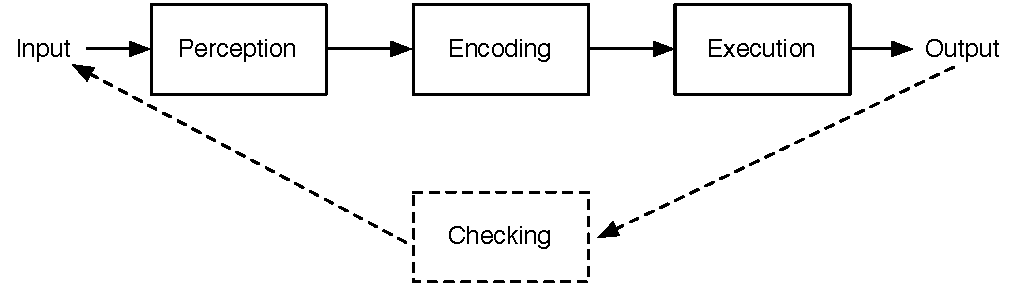
\includegraphics[width=0.8\textwidth]{images/background/HIP.pdf}
\caption[Different stages of a data entry task]{The different stages of a routine data entry task: a user perceives data input, encodes these in the mind, executes certain actions to enter data and produce the output, and can check the output against the original input.}
\vspace{-3pt}
\label{fig:ch2_hip}
\end{figure}


\subsection{The perception stage}
A data entry task begins with the user looking at the data that has to be entered on a data source.  The way in which data is presented to the user affects how that data is encoded by the user in the internal mind. The stronger data is encoded in memory, the more robust the user is against interruptions, and the less often the user may have to interrupt a task to look back at information. Several studies have shown that making information more difficult to perceive can encourage a deeper encoding in memory \citep{Diemand-Yauman2011, Soboczenski2013}. \citet{Soboczenski2013} conducted two experiments where people had to transcribe text and numbers that were presented either in a black font colour or a harder-to-read grey font colour. A hard-to-read font forced people to make more of an effort to read and understand the text, and as a result the text was more deeply processed and encoded in the mind. Participants made fewer data transcription errors if data was shown in the harder-to-read font colour, both for transcribing text and numbers. There was no difference in speed between the hard-to-read and normal font colour, suggesting that the improved accuracy was not due to a speed-accuracy trade-off. 

The way in which data is perceived and encoded is further influenced by how it is situated in the environment. The distributed cognition approach has been used as a theoretical framework to explain how cognition is ‘distributed’, meaning that people use a combination of internal information in their mind, and external information in the physical environment, to carry out work \citep{Hollan2000, Hutchins1995}. This means that to be able to understand how people work, it is not enough to know how the mind processes information, but it is also important to know how task information is situated in the physical world \citep{Hollan2000}. In most data entry studies, the data to enter is given to participants, which might not reflect how data entry is situated in offices. This motivates the need to understand how information for data entry work is spread in an office environment, which is the focus of the next chapter in this thesis. 

%\subsubsection{Summary}
%The first part of the data entry task entails the user perceiving the input.  A stronger representation of data in memory can improve task performance. Data may be strongly presented in memory because the data to enter is familiar to the user, but the design of the input source can also influence people's cognitive strategies and encourage a deeper encoding. Both internal and external information affect task performance, and where and how input is presented in the external environment affects people's internal representation of it. 

\subsection{The encoding stage}\label{sec:Encoding_stage}
After the user has perceived the input source in a data entry task, the next stage in the task sequence is the encoding stage, where data is encoded in memory. Prior work has shown several benefits of a deep encoding in memory: it can reduce interruptions to look back at information, but can also make people more robust against other, task-irrelevant, interruptions. As discussed earlier, another factor that  influences encoding is the costs associated with accessing data in the task environment. If information access costs increase, people rely on information in memory to avoid incurring costs to avoid making switches to the information source. \citet{Morgan2009} showed that in a copying task, if IAC was increased, participants made more of an effort to memorise the information. After an interruption, they were quicker to resume the task, because the pattern was still in memory. 

It is not just the external representation that influences how strongly something is encoded: in certain settings, certain data items are often re-used and thus are more strongly represented in memory. From text entry literature, it is known that words are easier to transcribe than non-words as they are used more often, they are more meaningful and thus have a stronger representation in memory \citep{Salthouse1986}. This highlights the importance to get a thorough understanding of the setting in which data entry is conducted. For example, \citet{Wiseman2013a} looked at number entry in hospitals and found some numbers were used far more often than others. Experiments showed that familiar numbers are faster to transcribe, suggesting that these are more strongly represented in memory than random numbers as well \citep{Wiseman2014} . This means that data entry interfaces that are intended for specific settings should be evaluated with familiar numbers used in that setting, rather than random numbers, and make it easier to enter commonly used numbers. 

%\subsubsection{Summary}
%At the second stage of the data entry task, the user processes the input in the mind. While usually designers aim to make it easy for people and not put too much cognitive load on the user, in some cases making the user process the information more deeply and adopt a memory-intensive strategy can have a positive effect on task performance. In the case of an interruption, taking time to remember where people were in the task sequence can reduce resumption errors. Furthermore, a deep encoding of data in memory can make people more accurate in data entry.

\subsection{The execution stage}
The third stage of the data entry task is the execution stage, which is the stage where the user performs the motoric actions to enter data into a device.

The design of the input method influences the speed with which users enter data, which can subsequently affect errors. \citet{Oladimeji2011} compared a number keypad with an incremental interface. The two types of interfaces are shown in Figure \ref{fig:interface-styles}. The number keypad is most common, and is used on calculators and phones. In this interface, each digit is assigned a button and additional buttons are usually a decimal point and a delete key to correct an error, as shown in Figure \ref{fig:numberpad}. In an incremental interface, a number is entered by increasing or decreasing the number using up and down keys. The incremental interface used in \citeauthor{Oladimeji2011}'s study is shown in Figure \ref{fig:incremental}. The double arrows increase and decrease the number by a larger amount than the single arrows. 

Results of the study showed that a number keypad allowed people to enter a number more quickly than an incremental interface, but more errors were made. With the keypad, the visual attention was more on the input keys than the display. In an incremental interface, people were changing an existing value rather than entering a new value, so they had to look at the display to see how their actions changed the current value. This attention on the display may have made it more likely for them to detect errors in time. While an incremental interface may not be feasible when entering large amounts of data as it will slow users down too much, it may be preferrable over a keypad in situations where accuracy is of great importance \citep{Thimbleby2011}. 

\begin{figure}[]
\begin{center}

\begin{subfigure}[b]{0.3\textwidth}
\centerline{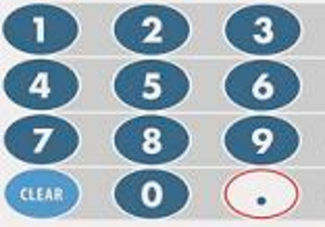
\includegraphics[scale=0.8]{images/background/numberpad.pdf}}
\caption{A number pad.}
\label{fig:numberpad}
\end{subfigure}
%\hfill%
\begin{subfigure}[b]{0.5\textwidth}
\centerline{
\includegraphics[scale=0.5]{images/background/incremental.pdf}}
\caption{An incremental interface.}
\label{fig:incremental}
\end{subfigure}

\caption[An incremental and keypad number entry interface.]{Two different number entry interfaces tested in \citeauthor{Oladimeji2011}'s study.}

\label{fig:interface-styles}
\end{center}
\end{figure}

%\subsubsection{Summary}
%At the third stage of the data entry task, the user inputs the data into a device. Data entry has a speed-accuracy tradeoff, and being able to enter data faster often come at the cost of an increased error rate. 
%Keyboards that slow people down may be useful in cases where accuracy is important, but may not be feasible in situations where a lot of data has to be entered. Depending on what users have to enter, shortcuts may get introduced in keyboard design so commonly used data can be entered quicker without the cost of increased errors. 

\subsection{The checking stage}
Most data transcription models consider the execution stage as the final stage of a data entry task \citep{Card1983, Salthouse1986}, but an additional stage can be a checking stage, where people review what they have entered and compare it with the original input, to see if it is correct. A reason why most models do not include this stage may be that people often do not make the effort to do so, and if they do, they are poor at detecting errors \citep{Olsen2008}. \citet{Olsen2008} conducted a lab experiment in which he simulated an internet banking tool, and participants were asked to enter account numbers from a paper sheet into a computer. After participants had entered an account number, they were presented with a confirmation screen with the input, and users were asked to check their input on this screen before submitting.  Participants confirmed 88 trials where they had entered an incorrect account number. In addition, in 178 trials the simulator changed people's input to another number and this incorrect number was presented on the confirmation screen. Only 5 of these 178 errors were detected and corrected. This large amount of incorrect confirmations again suggests users do not check properly, even if they are explicitly asked to do so. People are even worse at checking their input if they are switching between a data entry task and another task \citep{Wiseman2015}.

Given the limited effectiveness of confirmation screens \citep{Norman2002, Olsen2008}, some studies have supplemented these with lockouts, where users have to wait a short period of time before they are able to confirm and submit their input. While this has been shown to reduce errors in a controlled setting \citep{Gould2016b}, the presence of other tasks and distractions can entice users to switch to something else instead \citep{Gould2016b, Katidioti2013}.

\citet{Gould2016b} studied a number entry task where after each number the submit button would be disabled for a number of seconds, and a text instruction to check input appeared on the input screen.  This lockout was an effective method in encouraging people to check and detect errors in a lab setting. When the study was replicated online, a short lockout made people detect errors as well but the longer the lockout duration was, the more likely people were to switch to doing other tasks, and not check anymore. This illustrates the importance of taking the task context into account, and suggests that findings from controlled studies do not always directly translate to an applied setting \citep{Gould2016b}. 

Similar switching behaviour was found by \citet{Katidioti2013}. They conducted a lab experiment where people had to copy information and were interrupted by chat messages. Participants were free to choose when they wanted to attend to the messages. When people were locked out in the copying task and had to wait 3 seconds before they could enter the information, they often switched to the chat message, which made them forget the information to copy and slowed them down in completing the task.

%\subsubsection{Summary}
%After people have entered input, they can choose to check if what they have entered is correct. A popular method is visual checking, but people are poor at doing this, even if they are instructed to do so. It is possible to have people check, but the context needs to be considered. A lockout helped people check, but when possible to switch to other tasks people used the time to spend time on other tasks.

\subsection{Summary}
Research has shown how the way data is perceived, encoded, entered and checked all influence data entry performance. Time costs associated with perceiving data can improve encoding, and a better encoding leads to faster and more accurate entry.  The majority of data entry design interventions have been evaluated through laboratory experiments, and attempts to study data entry in a multitask setting suggest that people may interact with these interventions differently beyond a controlled setting. For example, in experimental studies the information was given and people were focused on the task, whereas many office settings are fragmented, and people can get distracted. How is data entry situated in an office setting? Are people focused on the task? And do they have the information readily available, or is this fragmented? In order to understand how people can be supported in making inquiries for data entry, it is important to understand how information for data entry is distributed in the environment.

\section{Conclusion}
This chapter reviewed literature on interruptions, information seeking and data entry. From this review, we learn that the length and timing affects the disruptiveness of interruptions, and that people try to avoid time costs in a controlled setting. As task-irrelevant interruptions are considered more disruptive than task-relevant interruptions, interruption management tools have mostly focused on avoiding these, even though relevant interruptions can be just as disruptive if not managed well. Furthermore, based on prior literature on information management we learn that how people search for information depends on the type of work. While existing tools support tasks where information sources need to be re-used, these provide no guidance of how to interrupt a task to collect information in the first place. Lastly, data entry research has shown that design interventions can reduce data entry errors if people are focused on the task, but that the context needs to be considered: people have workarounds to these design interventions if they (have to) interrupt and are exposed to distractions.

This highlights a need to better understand inquiries for a data entry task, and how the disruptiveness of these inquiries can be reduced. The next three chapters report a series of studies aimed to understand how interruption management tools can support people in managing inquiries for a routine data entry task, given variable time costs of required inquiries. To design a suitable tool, an understanding is required of how people currently self-interrupt for data entry work, which will be the focus of the next chapter.

%Based on prior work reviewed in this chapter, I make the hypothesis that disruptiveness can be reduced by reducing the length and number of interruptions, and by making interruptions at low workload moments in the task. I also make the hypothesis that people try to minimise time and that 

%Data entry follows four stages, and there are multiple strategies to complete the task, some being more accurate or efficient than others. Studies have shown that changing the design of a data entry interface can affect and improve how we enter data, and that different information access costs affect how often people visit the source from which to look up and enter data.

%It is not known yet how these data entry designs can be used in an office setting, where people have to manage multiple information sources with varying information access costs. Studies on office work have shown that work can be highly fragmented, and that people may often have to go in and out of several applications to complete their task. 
%In order to design interactive systems that truly support this type of data entry task, it is necessary to get a detailed understanding of the task in this setting, how users manage subtasks of looking up information for the data entry task, and to what extent the costs to access required resources affect their strategies.